\documentclass[11pt]{article}
\pdfoutput=1

\usepackage[T1]{fontenc}
\usepackage[utf8]{inputenc}
\usepackage[brazil]{babel} 
\usepackage{import}
\usepackage[toc,page]{appendix}
\usepackage{latexsym,amsfonts,amsmath,amssymb,mathrsfs,bbold,mathtools,esint,amsthm,mathtools,mathptmx}
\usepackage{dsfont}
\usepackage{mathtools}
\usepackage{float}
\usepackage{graphicx}
\usepackage{cite}
\usepackage{hyperref}
\usepackage{setspace}
\usepackage{color}
\usepackage{slashed}
\usepackage{cleveref}
\numberwithin{equation}{section}
\usepackage[colorinlistoftodos]{todonotes}
\usepackage[affil-it]{authblk}
\renewcommand\Authand{ e } 
\usepackage{float}
\usepackage{indentfirst}
\usepackage{soul}
\usepackage{booktabs}
\usepackage{eso-pic,graphicx}
\usepackage{nicefrac}
\usepackage{epsfig}
\usepackage[a4paper]{geometry}
\usepackage{makeidx}
\usepackage{fancyhdr}

\graphicspath{{/images}}

%--- PAGE LAYOUT >> PARA a4 COM ONESIDE ---
\usepackage{a4wide}
\topmargin 0in
%--- PAGE STYLE >> PARA a4 COM ONESIDE ---
  \pagestyle{fancy}                            
  \renewcommand{\sectionmark}[1]{%             %
    \markright{\thesection\ #1}}               %
  \fancyhf{}                                   % - limpar configurações
  \fancyhead[LE,RO]{\bfseries\thepage}         % - externo - número da página
  \fancyhead[LO]{\bfseries\nouppercase{\rightmark}}% - interno ímpar - seção
  \fancyhead[RE]{\bfseries\nouppercase{\leftmark}}% - interno par - capítulo
  \renewcommand{\headrulewidth}{0.5pt}         % - linha horizontal
  \renewcommand{\footrulewidth}{0pt}           %
  \addtolength{\headheight}{0.5pt}             % - espaço para a linha
  \fancypagestyle{plain}{%                     %
    \fancyhead{}                               % - sem cabeçalhos em páginas limpas
    \renewcommand{\headrulewidth}{0pt}         % - sem linhas
  }

\setcounter{MaxMatrixCols}{10}

\usepackage{color,hyperref}
\definecolor{darkblue}{rgb}{0.0,0.0,0.3}
\hypersetup{colorlinks,breaklinks,
            linkcolor=darkblue,urlcolor=darkblue,
            anchorcolor=darkblue,citecolor=darkblue}

\usepackage{palatino}

%%%%%% Comece a editar o arquivo a partir desta linha %%%%%%

\title{Características eletrônicas, síntese e aplicações de pontos quânticos}
\author[1]{Alan Abdalad Vianna\footnote{\href{mailto:alan@alunos.eel.usp.br}{alan@alunos.eel.usp.br}}}
\author[1]{Ângelo Augusto Santos Marcolin\footnote{\href{mailto:angelo.marcolin@usp.br}{angelo.marcolin@usp.br}} }
\author[1]{Bruno Sardinha Alves Pereira\footnote{\href{mailto:bruno.sap@alunos.eel.usp.br}{bruno.sap@alunos.eel.usp.br}} }
\author[1]{Caroline Teixeiera Lisboa\footnote{\href{mailto:caroline.tl@alunos.eel.usp.br}{caroline.tl@alunos.eel.usp.br}} }
\author[1]{Vitor Gabriel Fernandes\footnote{\href{mailto:vitor.gf@alunos.eel.usp.br}{vitor.gf@alunos.eel.usp.br}} }
\author[1]{Vinícius Rodrigues Costa\footnote{\href{mailto:vinicius.rc@alunos.eel.usp.br}{vinicius.rc@alunos.eel.usp.br}} }
\author[1]{Yasmin Michelin dos Santos\footnote{\href{mailto:yasmin.michelin@usp.br}{yasmin.michelin@usp.br}} }

\affil[1]{Escola de Engenharia de Lorena\\
Universidade de São Paulo\\
12602-810, Lorena, SP, Brasil}


\begin{document}
\onehalfspacing

\maketitle

\abstract{A sociedade nos dias atuais vive a era da nanotecnologia. Além dos dispositivos já existentes no mercado, há ainda uma enorme gama de novas nanotecnologias que prometem inovar e criar diversos dispositivos. Seja em áreas como medicina ou eletrônica, o uso de produtos nanotecnológicos se tornará cada vez mais comum. Em particular, há uma classe de nanopartículas semicondutoras, denominada ponto quântico, que vem chamando a atenção de diversos setores da indústria e pesquisa, devido às suas características únicas de confinamento. Dessa forma, o escopo da presente monografia é explicar o que são os pontos quânticos, suas propriedades e aplicações. Inicia-se introduzindo conceitos de mecânica quântica e física do estado sólido, base para entender fundamentos que descrevem semicondutores, além de possibilitar o entendimento das peculiaridades do ponto quântico quando comparado com um material \textit{bulk}. Em seguida, descreve-se o fenômeno de confinamento, uma das bases centrais  do trabalho, a equação de Brus e propriedades ópticas. Após a explanação acerca das características do ponto quântico, é feita uma descrição de forma sucinta sobre métodos de caracterização e síntese, além de aplicações dessas nanopartículas na área de tecnologia.}

\tableofcontents

\section{Introdução}
\par Pontos quânticos\cite{introducao1} são nanopartículas semicondutoras, que por terem o tamanho reduzido, se comportam como se estivesse sujeitas a um poço de potencial. Isso faz com que elétrons e buracos sofram um forte confinamento quântico nas três dimensões espaciais. Devido a esse confinamento, eles têm sua energia quantizada em valores discretos, como em um átomo. Por isso também são chamados de átomos artificiais.

\par A história dessas nanopartículas começa em 1980 em um artigo publicado pelo físico russo, Ekimov. Seu trabalho foi baseado no estudo de efeitos quânticos de tamanho em cristais semicondutores microscópicos em três dimensões. Segundo Ekimov \cite{introducao2}:

\begin{quote}
\textit{"Apresentamos a descoberta e a espectroscopia de uma nova classe de objetos que exibem efeitos quânticos de tamanho: cristais microscópicos tridimensionais de compostos semicondutores crescidos em uma matriz dielétrica transparente."}
\end{quote}

\par Apesar de tratar como uma nova classe de objetos, Ekimov não os denomida nem os trata como pontos quânticos.

\par Durante seu estudo, ao realizar a absorção espectral de três amostras de cristais microscópicos com raios diferentes, observou uma dependência na posição espectral das linhas de absorção, onde supôs se tratar de um efeito quântico de tamanho ocorrido devido ao tamanho da partícula, e complementa:

\begin{quote}
\textit{“Tais portadores de carga na matriz dielétrica estão presos em um poço de potencial onde as paredes são limitadas pelo cristal microscópico.”}
\end{quote}

\par Apesar de considerar esse poço de potencial simétrico e esférico, Ekimov não se aprofunda no tópico, deixando a discussão dos pontos quânticos como "um efeito quântico".

\par Foi apenas em 1984 que Louis Brus, ao apresentar uma relação entre o tamanho e o \textit{gap} de energia das nanopartículas semicondutoras após aplicar um modelo esférico na função de onda de um semicondutor \textit{bulk} para uma partícula, começa a dar forma ao conceito que futuramente será denominado ponto quântico.

\par No artigo\cite{introducao3}, Brus considera cristalitos suficientemente pequenos de modo que os níveis de energia \textit{bulk} não sejam válidos e afirma:

\begin{quote}
\textit{“Conforme os cristalitos se aproximam do tamanho da excitação 1S, as interações elétron-buraco com a superfície destes cristalitos dominam a dinâmica. Neste limite molecular, a energia dependerá do tamanho e forma dos cristalitos e da natureza do material.”}
\end{quote}

\par Apesar dos avanços nos estudos de Brus, levou cerca de uma década para que o ponto quântico voltasse a ser estudado, quando Murray\cite{introducao4}, durante seu estudo sobre evolução de propriedades de materiais pelo tamanho de cristalitos nanométricos, afirma que o regime de tamanhos intermediários dos cristalitos afetam o comportamento de materiais \textit{bulk}, emergindo a natureza discreta das propriedades moleculares deles.

\par O objetivo de Murray era estudar estes diferentes regimes para observar e, se possível, controlar certos comportamentos como efeitos ópticos de estados excitados altamente polarizados ou comportamento fotoquímico.

\par Já era conhecido que as propriedades físicas desses nanocristais semicondutores eram regidas por confinamentos espaciais de excitação e, apesar do progresso de certos semicondutores, a interpretação dos dados experimentais era complicada de ser analisada devido a problemas na superfície derivacional e baixa cristalinidade destes materiais.
     
\par Murray se concentrou na síntese e caracterização de nanocristais semicondutores de CdSe, devido às propriedades ópticas e eletroquímicas deste material, resultando futuramente em sínteses coloidais de compostos CdX (X = S, Se, Te) que permearam os estudos em pontos quânticos e suas aplicações.

\par As aplicações destes compostos foram se tornando cada vez mais amplas com o passar do tempo, porém, devido a toxicidade dos íons de Cádmio, ainda era inviável sua utilização na área biomédica.

\par A fim de melhorar a estabilidade dos núbleos de nanocristais para redução da toxicidade, passou-se a introduzir camadas de átomos de semicondutores com \textit{gap} de banda maior para encapsular o núcleo das nanopartículas, formando então nanocristais \textit{core-shell}. Como consequência desta mudança, a eficiência luminescente foi melhorada e estudada por Hines e Guyot-Sionnest em 1996 na caracterização da alta luminescência de nanocristais de CdSe encapsulados em ZnS.

\par Ao longo dos anos, foram realizadas melhorias como encapsulação dupla do núcleo, introdução de ácidos mercapto-carboxílicos que possibilitaram a solubilidade e eficiência fotoluminescente em solventes orgânicos e água, além de proporcionar uma gama de aplicações dos pontos quânticos.

\par Para entender melhor como os pontos quânticos podem ser utilizados nestas diversas aplicaçõoes, é necessário o entendimento de conceitos relacionados a mecânica quântica e física do estado sólido, que serão apresentados nas seções a seguir.

\section{Introdução à Mecânica Quântica e Física do Estado Sólido} %TODO: REFERENCIAR
\input{qm_fis.tex}

\section{Desenvolvimento}
\input{desenvolvimento.tex}

\section{Aplicação}
\subsection{Síntese de pontos quânticos}
A síntese de pontos quânticos pode ser realizada de diversas maneiras, dependendo da aplicação final e do próprio material. Neste capítulo serão apontados alguns dos métodos mais relevantes.

\subsubsection{Síntese de Pontos Quânticos Feitos de Carbono (CQDs)}

\par Os CQDs foram descobertos em 2004, e tem chamado atenção devido à sua ótima biocompatibilidade e propriedades de emissão de luz. Podem ser utilizados para produção de LEDs e bioimagens\cite{sintese1}.

\par Antes de iniciar a síntese de CQDs, é necessário saber que normalmente os procedimentos possuem três dificuldades\cite{sintese2}: junção de carboníferos durante a carbonização, controle do tamanho e uniformização dos CQDs e propriedades do meio de reação para a aplicação desejada. A junção de carboníferos pode ser evitada com tratamento químico e os outros dois problemas podem ser resolvidos tomando cuidado no preparo do meio de reação e no pós-tratamento – que não será estudado neste trabalho.

\par A síntese de CQDs pode ser feita por cinco principais métodos\cite{sintese2}. O primeiro, por separação química, consiste, basicamente, em uma sequência de tratamentos químicos com ácidos fortes. Suas vantagens são o preço acessível e a grande variabilidade de ácidos possíveis, enquanto que as desvantagens são principalmente a necessidade de várias etapas e o pouco controle do tamanho dos CQDs.

\par Um segundo processo é a síntese por carbonização eletroquímica. Nesse processo, lâminas de platina (Pt) podem ser usadas como eletrodos principal e auxiliares, enquanto um eletrodo saturado de calomelano (cloreto de mercúrio – $Hg_{2}Cl_{2}$) pode ser o eletrodo de referência. Os eletrodos são embebidos em uma solução que contém materiais de carbono \textit{bulk}. Nesse processo o tamanho dos CQDs é controlado pela diferença de potencial aplicada, contudo há poucos materiais de carbono \textit{bulk} disponíveis.

\par O outro processo possível é a separação à laser, que consiste em um alvo a base de carbono, suspenso em um solvente orgânico, vapor d’água e gás argônio (Ar), que é bombeado por uma irradiação a laser para que sejam formados os pontos quânticos. Nesse processo é fácil controlar as características do meio de reação, escolhendo o solvente orgânico correto. Contudo, o controle do tamanho dos pontos quânticos é mínimo.

\par Além dos processos já citados, há o procedimento de fabricação de CQDs a partir de irradiação de microondas. Nesse processo, a sacarose ($C_{12}H_{22}O_{11}$) é usada como fonte de carbonos e o dietilenoglicol como meio de reação. Apesar de ser um processo rápido (após apenas um minuto de irradiação já surgem CQDs que emitem ondas no comprimento da cor verde), há pouco controle do tamanho dos pontos quânticos.

\par O último processo é o de síntese por tratamento hidrotérmico. Nele uma solução orgânica, fornecedora de carbonos, como a glicose ($C_{6}H_{12}O_{6}$), o ácido cítrico ($C_{6}H_{8}O_{7}$), a quitosana, proteínas, ou até mesmo suco de banana, é colocada em um reator de alta temperatura, onde são formados os CQDs. Mesmo sendo um processo economicamente viável, possui baixo controle do tamanho dos CQDs criados.

\subsubsection{Síntese dos \textit{Core-Shell Quantum Dots} em Poros de Estruturas Metal-Orgânicas}

	\par Os pontos quânticos core-shell não são nada mais do que pontos quânticos revestidos por um outro material semicondutor que forma uma casca. Eles possuem inúmeras aplicações em diversas áreas, principalmente na biomedicina e em áreas com intensa utilização de propriedades fotovoltaicas. Seu estudo e aplicações obtiveram certa atenção na última década devido à sua relativa simplicidade de síntese e por possuírem um processo de fabricação barato [KLAUS]. Ademais, suas propriedades físicas podem ser facilmente ajustadas, variando o tamanho e a forma dos pontos quânticos.

	\par Um dos métodos de produção desses nanocristais semicondutores é por síntese confinada de CdSe em poros de estruturas metal-orgânicas (MOF)\cite{sintese3}. Tal método é ideal para uma síntese com grande densidade de pontos quânticos. Além disso, fazendo a escolha correta dos íons metálicos usados em junção com a liga orgânica mais adequada, é possível obter uma quantidade de poros razoável, com o tamanho e forma desejados. Além disso, as propriedades químicas dos poros podem ser ajustadas a fim de facilitar a nucleação dos pontos quânticos.

	\par Após o procedimento ser concluído, um escaneamento com o microscópio eletrônico de varredura (MEV) pode confirmar a síntese, como mostrado no exemplo da figura \ref{fig18}.

	\begin{figure}[H]
	  \centering
	  \caption{Microscopia no MEV de QDs de CdSe sintetizados em MOF\cite{sintese3}}
	  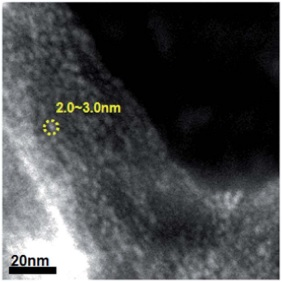
\includegraphics[width=0.65\textwidth]{images/figura18.jpg}
	  \label{fig18}
	\end{figure}

\subsubsection{Método de Caracterização}

	\par A seguir será apresentado três métodos não destrutivos de caracterização de pontos quânticos.

	\par \textbf{- Espectroscopia de Fotoluminescência}

		\par A espectroscopia de fotoluminescência\cite{sintese4} (PL) é uma técnica que utiliza a onda eletromagnética no espectro visível emitida por um material para sua caracterização, ou seja, para que se obtenham informações sobre determinadas propriedades de materiais.

		\par A radiação eletromagnética é incidida em geral por lasers sobre o material, o que excita os elétrons e os promove para a banda de condução, como visto anteriormente. Também foi visto que para que haja excitação é necessário que a energia do fóton incidente seja igual ou maior que a energia de \textit{gap}, o que faz com que o material absorva esse fóton. Quando os elétrons voltam ao seu estado normal pode haver uma emissão de radiação eletromagnética, o que é chamado de processo radiativo. Somente o processo radiativo será computado no espectro de emissão, pois as recombinações não radiativas serão dissipadas dentro da superfície do material\cite{sintese4}.

		\par A energia emitida através de um fóton numa transição direta é dada por $hv$, como ilustrado na figura \ref{fig19}.

		\begin{figure}[H]
		  \centering
		  \caption{Representação a absorção do fóton para a criação do éxciton.\cite{sintese5}}
		  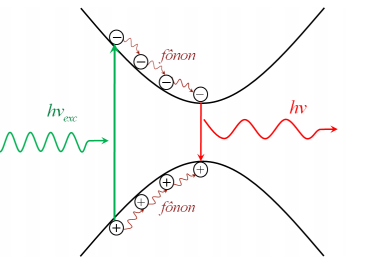
\includegraphics[width=0.65\textwidth]{images/figura19.png}
		  \label{fig19}
		\end{figure}


		\par Com a espectroscopia de fotoluminescência, algumas variáveis podem ser tiradas de uma espectroscopia de PL dos pontos quânticos coloidais, tais como: o comprimento de onda do máximo de emissão, a largura a meia altura do espectro e a intensidade de emissão. Esses espectros, após análise de dados,  remetem a informação sobre os tamanhos dos pontos quânticos, suas distribuições de tamanhos e sua eficiência de emissão de luz, respectivamente. 

		\par A figura \ref{fig20} mostra espectro de PL de pontos quânticos coloidais de três materiais e com tamanhos diferentes.

		\begin{figure}[H]
		  \centering
		  \caption{Microscopia no MEV de QDs de CdSe sintetizados em MOF\cite{sintese3}}
		  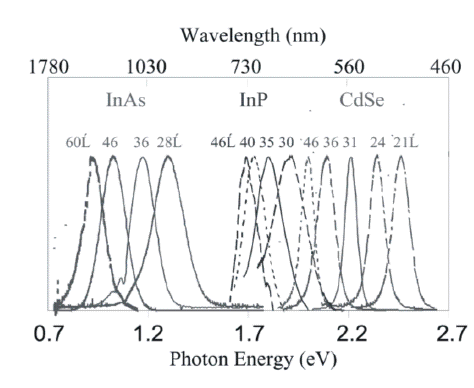
\includegraphics[width=0.65\textwidth]{images/figura20.png}
		  \label{fig20}
		\end{figure}

		\par Nota-se ao ver os espectros de PL que o tamanho dos pontos quânticos modifica  comprimento máximo de emissão e a energia associada. Como foi visto teoricamente em propriedades ópticas.

	\par \textbf{- Absorção Óptica}

		\par A absorção óptica é uma análise que se dá pela quantidade de luz absorvida pelo material. A quantidade de luz incidente é diferente da transmitida, seguindo a lei de Lambert-Beer.

		\begin{equation}
			\label{sintese_1}
			A = L\beta d = \log \left(\frac{I_{0}}{I} \right),
		\end{equation}
		onde $L$ é o tamanho óptico que a luz percorre, $\beta$ é o coeficiente de absortividade e $d$ é a concentração da amostra.

		\par O principal motivo para que se analise os espectros de absorção é obter experimentalmente a energia de \textit{gap} das nanoestruturas, a qual pode ser obtida traçando uma reta tangente à borda de absorção fundamental na região do limiar de absorção (onset absorption). O intercepto desta reta tangente com o eixo dos comprimentos de onda nos leva ao comprimento de onda do limiar de absorção ($\lambda$), chegando na equação:

		\begin{equation}
			\label{sintese_2}
			E_{onset} = \frac{hc}{\lambda_{onset}} = E_{gap}.
		\end{equation}

		\par Esse conceito é visto no espectro de absorção abaixo:

		\begin{figure}[H]
		  \centering
		  \caption{Obtenção do comprimento de onda do limiar de absorção de uma amostra\cite{confinamento5}.}
		  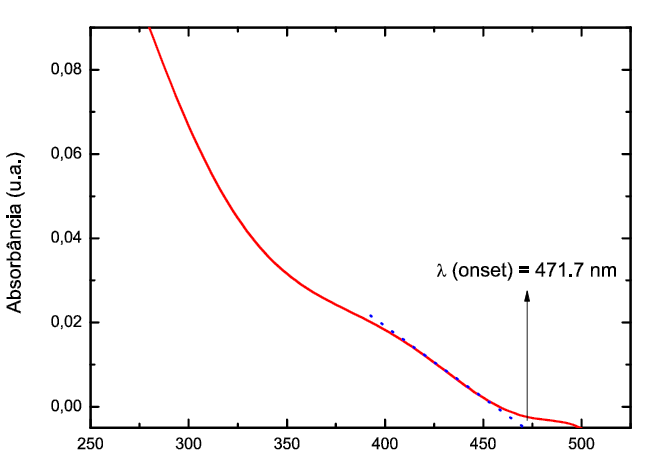
\includegraphics[width=0.65\textwidth]{images/figura21.png}
		  \label{fig21}
		\end{figure}

		\par Outra análise que se obtém pela absorção óptica é o confinamento em alguma direção. O espectro da absorção é deslocado para o azul caso haja esse confinamento. Esse deslocamento dos espectros está relacionado ao tamanho dos pontos quânticos, de modo que quanto menor for o comprimento de onda menor será o tamanho os pontos quânticos\cite{sintese5}.

	\par \textbf{- Espectroscopia Raman}

		\par A espectroscopia dispersão de polarização de Raman caracteriza os pontos quânticos sintetizados pelo método eletroquímico. O método de Raman possibilita a sondagem de estruturas eletrônicas confinadas de pontos quânticos\cite{sintese7}.

		\begin{figure}[H]
		  \centering
		  \caption{Exemplo de espectroscopia Raman\cite{sintese7}}
		  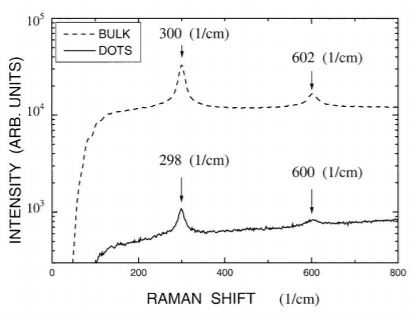
\includegraphics[width=0.65\textwidth]{images/figura22.jpg}
		  \label{fig22}
		\end{figure}

		\par No exemplo da figura \ref{fig22}, todo o espectro está sendo excitado com um feixe de laser de 514 nm de Argônio que corresponde a uma energia de $2.4eV$, enquanto a energia do \textit{gap} de banda do CdS é aproximadamente $3eV$. Essa proximidade de energias provoca uma ressonância no sistema que afeta a onda emitida pelo ponto quântico. Parte da energia inserida é refletida, parte é absorvida pelo sistema e parte sofre um espalhamento dentro do material\cite{sintese7}.

		\par A radiação, ao atingir a amostra, é espalhada e adquire uma nova energia. Esse efeito é chamado de espalhamento inelástico e é conhecido como efeito Raman. A partir da análise dessa energia é que se obtém informações sobre o material, tais como definição da orientação cristalográfica. Com o gráfico obtido pela análise Raman é possível analisar a estrutura dos materiais, e isso é útil no caso dos pontos quânticos para que se analisem os efeitos da mudança de tamanho nesse tipo de material\cite{sintese5}.

\subsubsection{Aplicações de pontos quânticos}

	\par Os pontos quânticos possuem diversas aplicações em muitas áreas devido às suas propriedades. Algumas dessas áreas são: biomedicina, energia sustentável, eletrônica e óptica.  Neste trabalho, apresentaremos de forma breve algumas dessas aplicações.

	\par \textbf{- Biomedicina}

		\par O fenômeno de fluorescência dos pontos quânticos pode ser utilizado na área de biomedicina como marcadores fluorescentes em moléculas e células biológicas, como proteínas e DNA, já que podem se ligar facilmente à essas moléculas. Os marcadores servem nesse sentido para observar o comportamento dessas moléculas dentro de uma amostra, através da irradiação de luz pelo ponto quântico\cite{bulk2}. Os marcadores fluorescentes de pontos quânticos apresentam muitas vantagens quando comparados com marcadores de corantes orgânicos, como por exemplo, são cerca de vinte vezes mais brilhantes e possuem mais fotoestabilidade, sendo cem vezes mais resistente a fotobranqueamento\cite{sintese8}.

		\par Um exemplo da eficiência dos pontos quânticos na área médica é analisado a seguir. Na figura \ref{fig23}a apresenta os espectros de absorção e em \ref{fig23}b de emissão das substâncias Rodoamina 6G e de um ponto quântico de CdSe. Observa-se que o espectro de emissão do QD é mais estreito que o da Rodoamina 6G e que seu perfil de absorção é mais amplo e contínuo, o que significa que o ponto quântico consegue ser melhor excitado em qualquer comprimento de onda inferior à aproximadamente $530nm$ e emite radiação eletromagnética de maneira mais precisa.

		\begin{figure}[H]
		  \centering
		  \caption{Espectro da Rodoamina 6G, onde (a) é o espectro de absorção e (b) de emissão.\cite{sintese9}}
		  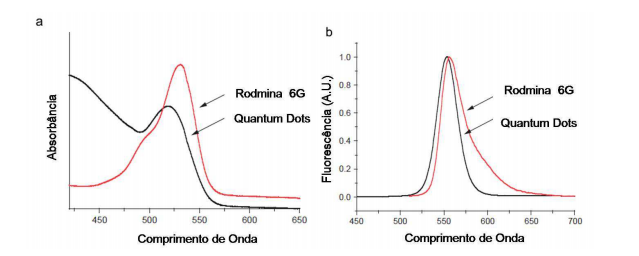
\includegraphics[width=0.95\textwidth]{images/figura23.png}
		  \label{fig23}
		\end{figure}

	\par \textbf{- Televisões de ponto quântico}

		\par O que faz a televisão de ponto quântico ser tão atraente são as propriedades ópticas devido ao confinamento quântico. Como visto, ao fornecer energia num comprimento de onda na faixa do ultravioleta, os elétrons nos pontos quânticos são excitados, saltam de banda e quando retornam emitem um fóton. Esse fóton tem um comprimento de onda bem definido devido à discretização do elétron, e o comprimento de onda é determinado pelo tamanho do ponto quântico\cite{bulk2}. A característica de ter um comprimento de onda bem definido é uma das características mais importantes para gerar uma imagem de boa qualidade.
		
		A televisão de ponto quântico é LCD (Liquid Crystal Display) e, sucintamente, pode-se dizer que a televisão é composta de duas partes principais que são uma luz de fundo, denominada backlight, e um display de cristal líquido, também conhecido como LCM (liquid-crystal module)\cite{sintese10}. O backlight é responsável por gerar uma luz branca que passará no LCM. O LCM é composto por milhões de pixels, sendo que um pixel é composto por subpixels de cores azul, vermelho e verde\cite{sintese10}. O pixel determina a tonalidade da cor que se deseja reproduzir através da combinação das três cores primárias, e quando a luz branca passa pelo pixel, ele reproduz a tonalidade e é possível ver, através do conjunto de todos os pixels, a imagem na televisão\cite{sintese10}.

		Os pontos quânticos compõe o backlight gerando luz branca pela combinação de três pontos quânticos de tamanhos diferentes e que emitem luz em comprimentos de onda na faixa do vermelho, azul e verde\cite{sintese11}. Para que os pontos quânticos emitam fótons é necessário que eles absorvam fótons de uma fonte de LED no comprimento de onda ultravioleta. A luz branca possui uma pureza muito maior comparada a televisões que possuem backlight de LED de materiais \textit{bulk}, porque esta é formada através da combinação de LED azul com fósforo YAG (yttrium-aluminum-garnet), criando um conjunto de espectros que contém mais comprimentos de onda na faixa no azul e no amarelo, e bem pouco na faixa do vermelho e verde\cite{sintese10}. Como consequência, a luz de fundo de LED de material \textit{bulk}, quando em contato com os pixels, não gera tons de cores como geraria se fosse uma luz essencialmente branca, como é criado pelos pontos quânticos.

		Um comparativo pode ser feito entre a televisão de LED e de ponto quântico. Uma das formas de quantificar o espectro de cores que uma televisão consegue atingir é através do diagrama de cromaticidade, criado pela CIE (Comissão Internacional de Iluminação), no qual é apresentado um diagrama com todas as cores que podem ser detectadas pelo olho humano. Como mencionado, no LMC se utiliza o sistema RGB, que é uma combinação das cores vermelho, verde e azul para gerar as cores que aparecem na televisão\cite{sintese11}. Essas cores estão contidas dentro de um triângulo, e os vértices do triângulo são as cores RGB. A Figura 1 apresenta o triângulo correspondente à televisão de LED e a Figura \ref{fig24}, da televisão de ponto quântico\cite{sintese12}. Quanto maior o triângulo, mais cores podem ser reproduzidas pelo display. A televisão de ponto quântico apresenta um triângulo maior comparada a televisões de LED já presentes no mercado, pois os pontos quânticos liberam fótons com um espectro de largura bem pequena, entre $20 e 35nm$, que corresponde a espectros próximos de cores saturadas, que ficam na borda do diagrama de cromaticidade\cite{sintese11}.

		\begin{figure}[H]
		  \centering
		  \caption{a) Triângulo que representa a escala de cores em televisões de LED. b) Triângulo em linha contínua representa escala de cores dada por Adobe RGB e o triângulo pontilhado é a escala de cores da televisão de ponto quântico.\cite{sintese12}}
		  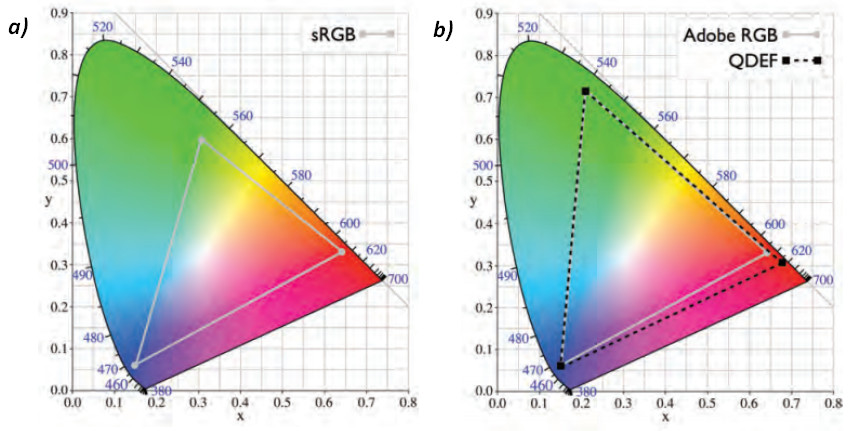
\includegraphics[width=0.65\textwidth]{images/figura24.jpg}
		  \label{fig24}
		\end{figure}
  

\phantomsection
\addcontentsline{toc}{section}{Referências}
\begin{thebibliography}{99}
% INTRODUÇÃO
\bibitem{introducao1} de Figueiredo Oliveira, André Rezende. \href{http://www.infis.ufu.br/sites/infis.ufu.br/files/Anexos/Bookpage/TCC%20F%C3%8DSICA%20DE%20MATERIAIS%202009_2%20-%20ANDRE%20REZENDE.pdf}
{\it Caracterização Óptica de Pontos Quânticos Semicondutores de CdS em Matrizes Poliméricas}. 
\bibitem{introducao2} Ekimov, Alexey I., and Alexei A. Onushchenko. \href{https://www.researchgate.net/profile/Alexey_Onushchehko/publication/234289541_Quantum_Size_Effect_in_Three-Dimensional_Microscopic_Semiconductor_Crystals/links/0c9605305fa93c4e3d000000.pdf}{\it Quantum size effect in three-dimensional microscopic semiconductor crystals}. Jetp Lett 34.6 (1981): 345-349.
\bibitem{introducao3} Brus, Louis E. \href{http://aip.scitation.org/doi/10.1063/1.447218}{\it Electron-electron and electron-hole interactions in small semiconductor crystallites: The size dependence of the lowest excited electronic state}. The Journal of chemical physics 80.9 (1984): 4403-4409.
\bibitem{introducao4} Murray, CBea, David J. Norris, and Moungi G. Bawendi. \href{http://pubs.acs.org/doi/abs/10.1021/ja00072a025?journalCode=jacsat}{\it Synthesis and characterization of nearly monodisperse CdE (E= sulfur, selenium, tellurium) semiconductor nanocrystallites}. Journal of the American Chemical Society 115.19 (1993): 8706-8715.
\bibitem{introducao5} Zhu, Jun-Jie, et al. \href{https://link.springer.com/book/10.1007/978-3-642-44910-9}{\it Quantum dots for DNA biosensing. Vol. 165}. Springer, 2013.

% INTRODUÇÃO A MECÂNICA QUÂNTICA E FÍSICA DO ESTADO SÓLIDO
  %Redes Cristalinas
\bibitem{qm_fis0} Koole, Rolf, et al. \href{https://link.springer.com/chapter/10.1007/978-3-662-44823-6_2}{\it Size effects on semiconductor nanoparticles}. Nanoparticles. Springer Berlin Heidelberg, 2014. 13-51.
\bibitem{qm_fis1} Band, Yehuda B., and Yshai Avishai. \href{https://www.elsevier.com/books/quantum-mechanics-with-applications-to-nanotechnology-and-information-science/band/978-0-444-53786-7}{\it Quantum mechanics with applications to nanotechnology and information science. Academic Press, 2013}.
\bibitem{qm_fis2} Oliveira, Ivan S., and Vitor LB De Jesus. \href{http://www.saraiva.com.br/introducao-a-fisica-do-estado-solido-2-ed-3527998.html}{\it Introdução à física do estado sólido}. Editora Livraria da Fisica, 2005.
\bibitem{heterojuncao} Margaritondo, Giorgio, ed. \href{http://www.springer.com/br/book/9789027728234}{\it Electronic structure of semiconductor heterojunctions}. Vol. 1. Springer Science \& Business Media, 2012.
  %Equação de Schrödinger
\bibitem{qm_fis3} Eisberg, Robert Martin; Resnick, Robert - \href{https://www.livrariadafisica.com.br/detalhe_produto.aspx?id=6237}{\it Física Quântica}
\bibitem{qm_fis4} C.W. Sherwin- \href{https://www.amazon.com/Introduction-Quantum-Mechanics-C-W-Sherwin/dp/0030068851}{\it Introduction to quantum mechanics} - Holt, Rinehart \& Winston of Canada Ltd (1959). 
\bibitem{qm_fis5} Ashcroft, Neil W., and N. David Mermin. \href{https://www.livrariadafisica.com.br/detalhe_produto.aspx?id=101883}{\it Física do estado sólido}. Cengage Learning, 2011.
\bibitem{qm_fis6} Kittel, Charles. \href{https://www.amazon.com.br/dp/8521615051/ref=asc_df_85216150515016109?smid=A1ZZFT5FULY4LN&tag=goog0ef-20&linkCode=asn&creative=380341&creativeASIN=8521615051}{\it Introdução à física do estado sólido}. Grupo Gen-LTC, 2006.
\bibitem{qm_fis7} Thompson, D. \href{http://aapt.scitation.org/doi/abs/10.1119/1.18243}{\it The reciprocal lattice as the Fourier transform of the direct lattice}. American Journal of Physics 64.3 (1996): 333-334.
\bibitem{qm_fis8} Wang, Gwo-Ching, and Toh-Ming Lu. \href{https://books.google.com.br/books?hl=pt-BR&lr=&id=LEC9BAAAQBAJ&oi=fnd&pg=PR6&dq=ISBN:+978-1-4614-9286-3&ots=6N688QVTZa&sig=eKxt-la7NjrX5ZWrmHEoIZpaTwQ#v=onepage&q=ISBN%3A%20978-1-4614-9286-3&f=false}{\it RHEED Transmission Mode and Pole Figures: Thin Film and Nanostructure Texture Analysis}. Cap. 2. Springer Science \& Business Media, 2013.
\bibitem{qm_fis9} I. Prigogine, Stuart A. Rice. \href{http://onlinelibrary.wiley.com/book/10.1002/9780470142813}{\it Advances in Chemical Physics, Volume 57}. Wiley Interscience, 2007.
\bibitem{qm_fis10} Dagotto, Elbio. \href{http://www.springer.com/la/book/9783540432456} {\it Nanoscale Phase Separation and Colossal Magnetoresistance: The Physics of Manganites and Related Compounds}. Springer-Verlag Berlin Heidelberg, 2003 
\bibitem{qm_fis11} Rodrigues, Rafael de Lima. \href{http://sbfisica.org.br/rbef/pdf/v19_68.pdf}{\it Mecânica Quântica na Descrição de Schrödinger}. Revista Brasileira de Ensino de Física, vol. 19, n 1, p.68-83, 1997

% FRUSTRADO - TODO: Mudar links
 \bibitem{frustrado1} Eisberg, Robert Martin Resnick, and Cota Araiza Robert. \href{http://gen.lib.rus.ec/book/index.php?md5=80CCC290E6FFF645ADF0BA24178E4C5D}{\it Física cuántica: átomos, moléculas, sólidos, núcleos y partículas. 1994}.
 \bibitem{frustrado2} Atkins, Peter, and Loretta Jones. \href{http://gen.lib.rus.ec/book/index.php?md5=6D32E94CECA0A9BD6FFF5F1307078071}{\it Chemical principles: The quest for insight. Macmillan, 2007}.
 \bibitem{frustrado3} Peter, Y. U., and Manuel Cardona. \href{http://gen.lib.rus.ec/book/index.php?md5=20A8507AB491C812ED2C75D08740987A}{\it Fundamentals of semiconductors: physics and materials properties}. Springer Science \& Business Media, 2010.
 \bibitem{frustrado5} Dagotto, Elbio. \href{http://gen.lib.rus.ec/book/index.php?md5=3C621FEBFE1EBBF8B376CED188D04A84}{\it Nanoscale phase separation and colossal magnetoresistance: the physics of manganites and related compounds. Vol. 136}. Springer Science \& Business Media, 2013.
 \bibitem{frustrado6} de Lima Rodrigues, Rafael. \href{http://sbfisica.org.br/rbef/pdf/v19_68.pdf}{\it Mecânica Quântica na Descrição de Schrödinger.} Revista Brasileira de Ensino de Física 19.1, 1997.
 \bibitem{frustrado7} Zill, Dennis G., and Michael R. Cullen. \href{http://gen.lib.rus.ec/book/index.php?md5=8673E58CC84FED5F909BEA1CC2BC4E3F}{\it Differential Equations With Boundary-Value Problems}. Thomson Brooks/Cole, 1996.
 % Potencial Periódico e Teorema de Bloch
 \bibitem{bloch1} Silva, Jusciane da Costa e. \href{www.repositorio.ufc.br/bitstream/riufc/12669/1/2008_tese_jcsilva.pdf}{\it Confinamento Quântico em Hetero-estruturas Semicondutoras de Baixa Dimensionalidade}. Universidade Fedaral do Ceará, 2008.
 \bibitem{bloch2} H. Ibach and Hans Lüth, \href{http://www.springer.com/us/book/9783540938033}{\it Solid-State Physics: An Introduction to Principles of Materials Science}, Springer-Verlag, 2nd Ed., 1995
% Semicondutores Bulk
\bibitem{bulk1} Averill, B. A., and P. Eldredge. \href{https://2012books.lardbucket.org/books/principles-of-general-chemistry-v1.0m/index.html}{\it Principles of General Chemistry (v. 1.0)}. Creative Commons licensed (2012): 2991.
\bibitem{bulk2} Sattler, Klaus D. \href{https://www.amazon.com/Handbook-Nanophysics-Nanoparticles-Quantum-Dots-ebook/dp/B008I9VLAI}{\it Handbook of Nanophysics: Nanoparticles and Quantum Dots}. CRC Press, 2016.
%Confinamento
\bibitem{confinamento1} Yoffe, A. D. \href{http://adsabs.harvard.edu/abs/1993AdPhy..42..173Y}{\it Low-dimensional systems: quantum size effects and electronic properties of semiconductor microcrystallites (zero-dimensional systems) and some quasi-two-dimensional systems}. Advances in Physics, vol. 42, Issue 2, p.173-262, 1993
\bibitem{confinamento2} Dick, Rainer. \href{http://www.springer.com/us/book/9781489990686}{\it Advanced Quantum Mechanics: Materials and Photons}. Springer-Verlag New York, 2012
\bibitem{confinamento3} Harrison, Paul \href{http://www.wiley.com/WileyCDA/WileyTitle/productCd-0470010819.html}{\it Quantum Wells, Wires and Dots: Theoretical and Computational Physics of Semiconductor Nanostructures}. Wiley, 2005
\bibitem{confinamento4} Ephrem O. Chukwuocha, Michael C. Onyeaju, Taylor S. T. Harry. \href{http://file.scirp.org/pdf/WJCMP20120200011_36451105.pdf}{\it Theoretical Studies on the Effect of Confinement on Quantum Dots Using the Brus Equation}. World Journal of Condensed Matter Physics, 2012, 2, 96-100.
\bibitem{confinamento5} Maronesi, Ray Nascimento. \href{http://www.locus.ufv.br/handle/123456789/9775}{\it Nova técnica para síntese de pontos quânticos coloidais de CdS em meio puramente aquoso}. Universidade Federal de Viçosa, 2016
%Aplicações Opticas
\bibitem{optica1} Melville, Jonathan. \href{https://www.ocf.berkeley.edu/~jmlvll/lab-reports/quantumDots/quantumDots.pdf}{\it Optical Properties of Quantum Dots}. UC Berkeley College Of Chemistry, 2015
\bibitem{optical2} Jones, Aaron, and Nick Verlinden. \href{https://web.wpi.edu/Pubs/E-project/Available/E-project-042607-125225/unrestricted/QuantumDots.pdf}{\it Optical Properties of Quantum Dots: An Undergraduate Physics Laboratory}. 2007.
%Aplicações Sintese
\bibitem{sintese1} Machado, Claudia Emanuele, et al. \href{https://www.researchgate.net/profile/Marco_Schiavon2/publication/279939933_Carbon_Quantum_Dots_Chemical_Synthesis_Properties_and_Applications/links/559fe9f908aed84bedf44826.pdf}{\it Pontos Quânticos de Carbono: Síntese Química, Propriedades e Aplicações}. Revista Virtual de Química 7.4 (2015): 1306-1346.
\bibitem{sintese2} Wang, Youfu, and Aiguo Hu. \href{http://www.rsc.org/chemical-sciences-repository/articles/article/dr000000002036?doi=10.1039%2Fc4tc00988f}{\it Carbon quantum dots: synthesis, properties and applications}. Journal of Materials Chemistry C 2.34 (2014): 6921-6939.
\bibitem{sintese3} Wakaoka, Takuo, et al. \href{http://pubs.rsc.org/en/content/articlelanding/2014/tc/c4tc01136h#!divAbstract}{\it Confined synthesis of CdSe quantum dots in the pores of metal–organic frameworks}. Journal of Materials Chemistry C 2.35 (2014): 7173-7175.
\bibitem{sintese4} da Silva, Isaías Ferreira. \href{http://www.dsif.fee.unicamp.br/~furio/IE607A/Pl.pdf}{\it Medidas de Caracterização e Análise de Materiais: Espectroscopia De Fotoluminescência}. 2000.
\bibitem{sintese5} Neto, Ernesto Soares de Freitas. \href{https://repositorio.ufu.br/bitstream/123456789/15607/1/ErnestoSoares.pdf}{\it Estudo de Pontos Quânticos Semicondutores e Semimagnéticos}. Universidade Federal de Uberlândia, 2013.
\bibitem{sintese6} Rodrigues, Ariano De Giovanni., José Cláudio Galzerani. \href{http://www.scielo.br/scielo.php?script=sci_arttext&pid=S1806-11172012000400009&lng=pt&tlng=pt}{\it Espectroscopias de infravermelho, Raman e de fotoluminescência: potencialidades e complementaridades}. Rev. Bras. Ensino Fís. vol.34 no.4 São Paulo out. 2012.
\bibitem{sintese7} A. Balandin, K. L. Wang, N. Kouklin, S. Bandyopadhyay. \href{http://sci-hub.cc/10.1063/1.125681}{\it Raman spectroscopy of electrochemically self-assembled CdS quantum dots}. Applied Physics Letter Volume76, Number 2, 2000.
\bibitem{sintese8} Fontes, Adriana, and Beate Saegesser Santos, eds. \href{http://www.springer.com/gp/book/9781493912797}{\it Quantum dots: applications in biology}. Springer New York, 2014.
\bibitem{sintese9} Raele, Renata Almeida. \href{http://repositorio.ufpe.br/bitstream/handle/123456789/12231/Disserta\%C3\%A7ao\%20Renata\%20Raele.pdf?sequence=1\&isAllowed=y}{\it AVALIAÇÃO DA CITOTOXICIDADE DE QUANTUM DOTS, IN VITRO, EM CÉLULAS RAW 264.7}. Universidade Federal de Pernambuco, 2013.
\bibitem{sintese10} Chen, Jian, Veeral Hardev, and Jeff Yurek. \href{https://www.researchgate.net/publication/291313785_Quantum-dot_displays_Giving_LCDs_a_competitive_edge_through_color}{\it Quantum Dot Displays: Giving LCDs a Competitive Edge Through Color}. Nanotech. L. \& Bus. 11 (2014): 4.
\bibitem{sintese11} Talapin, Dmitri V., and Jonathan Steckel. \href{https://www.cambridge.org/core/journals/mrs-bulletin/article/quantum-dot-lightemitting-devices/94FDE7F4EF98D19F4B78E2AD2F656C4F}{\it Quantum dot light-emitting devices}. Mrs Bulletin 38.09 (2013): 685-691.
\bibitem{sintese12} Han, Hau-Vei, et al. \href{https://www.osapublishing.org/oe/abstract.cfm?uri=oe-23-25-32504}{\it Resonant-enhanced full-color emission of quantum-dot-based micro LED display technology}. Optics express 23.25 (2015): 32504-32515.
 \end{thebibliography}
\end{document}
